\documentclass[twocolumn]{article}

\title{Evaluation}
\usepackage{graphicx}
\usepackage[margin=0.75in]{geometry}

\graphicspath{ {graphs/} }

\addtolength{\topmargin}{0.25in}
	\addtolength{\textheight}{-0.5in}

\begin{document}


\begin{center}
\section*{Empirical Evaluation}
\end{center}


\paragraph{•}
	We tested Flair's performance in relation to the following questions:\\
	\textbf{Question 1:} How does Flair compare to other inter-application communication analysis tools in respect to the amount of time it takes to analyze a bundle of applications?\\
	\textbf{Question 2:} How does Flair compare to other tools with respect to the number of applications it fails to analyze?\\
	\textbf{Question 3:} How accurately does Flair analyze vulnerabilities within applications when ran against a bundle of benchmark applications?\\
	\textbf{Question 4:} How does Flair's accuracy in analyzing applicaions compare to other inter-application analysis tools?\\
	
	
	\subparagraph{Covert}
		Jianghao probably explained this already
	\subparagraph{DidFail}
		Jianghao probably explained this already


		\begin{figure}[h]
			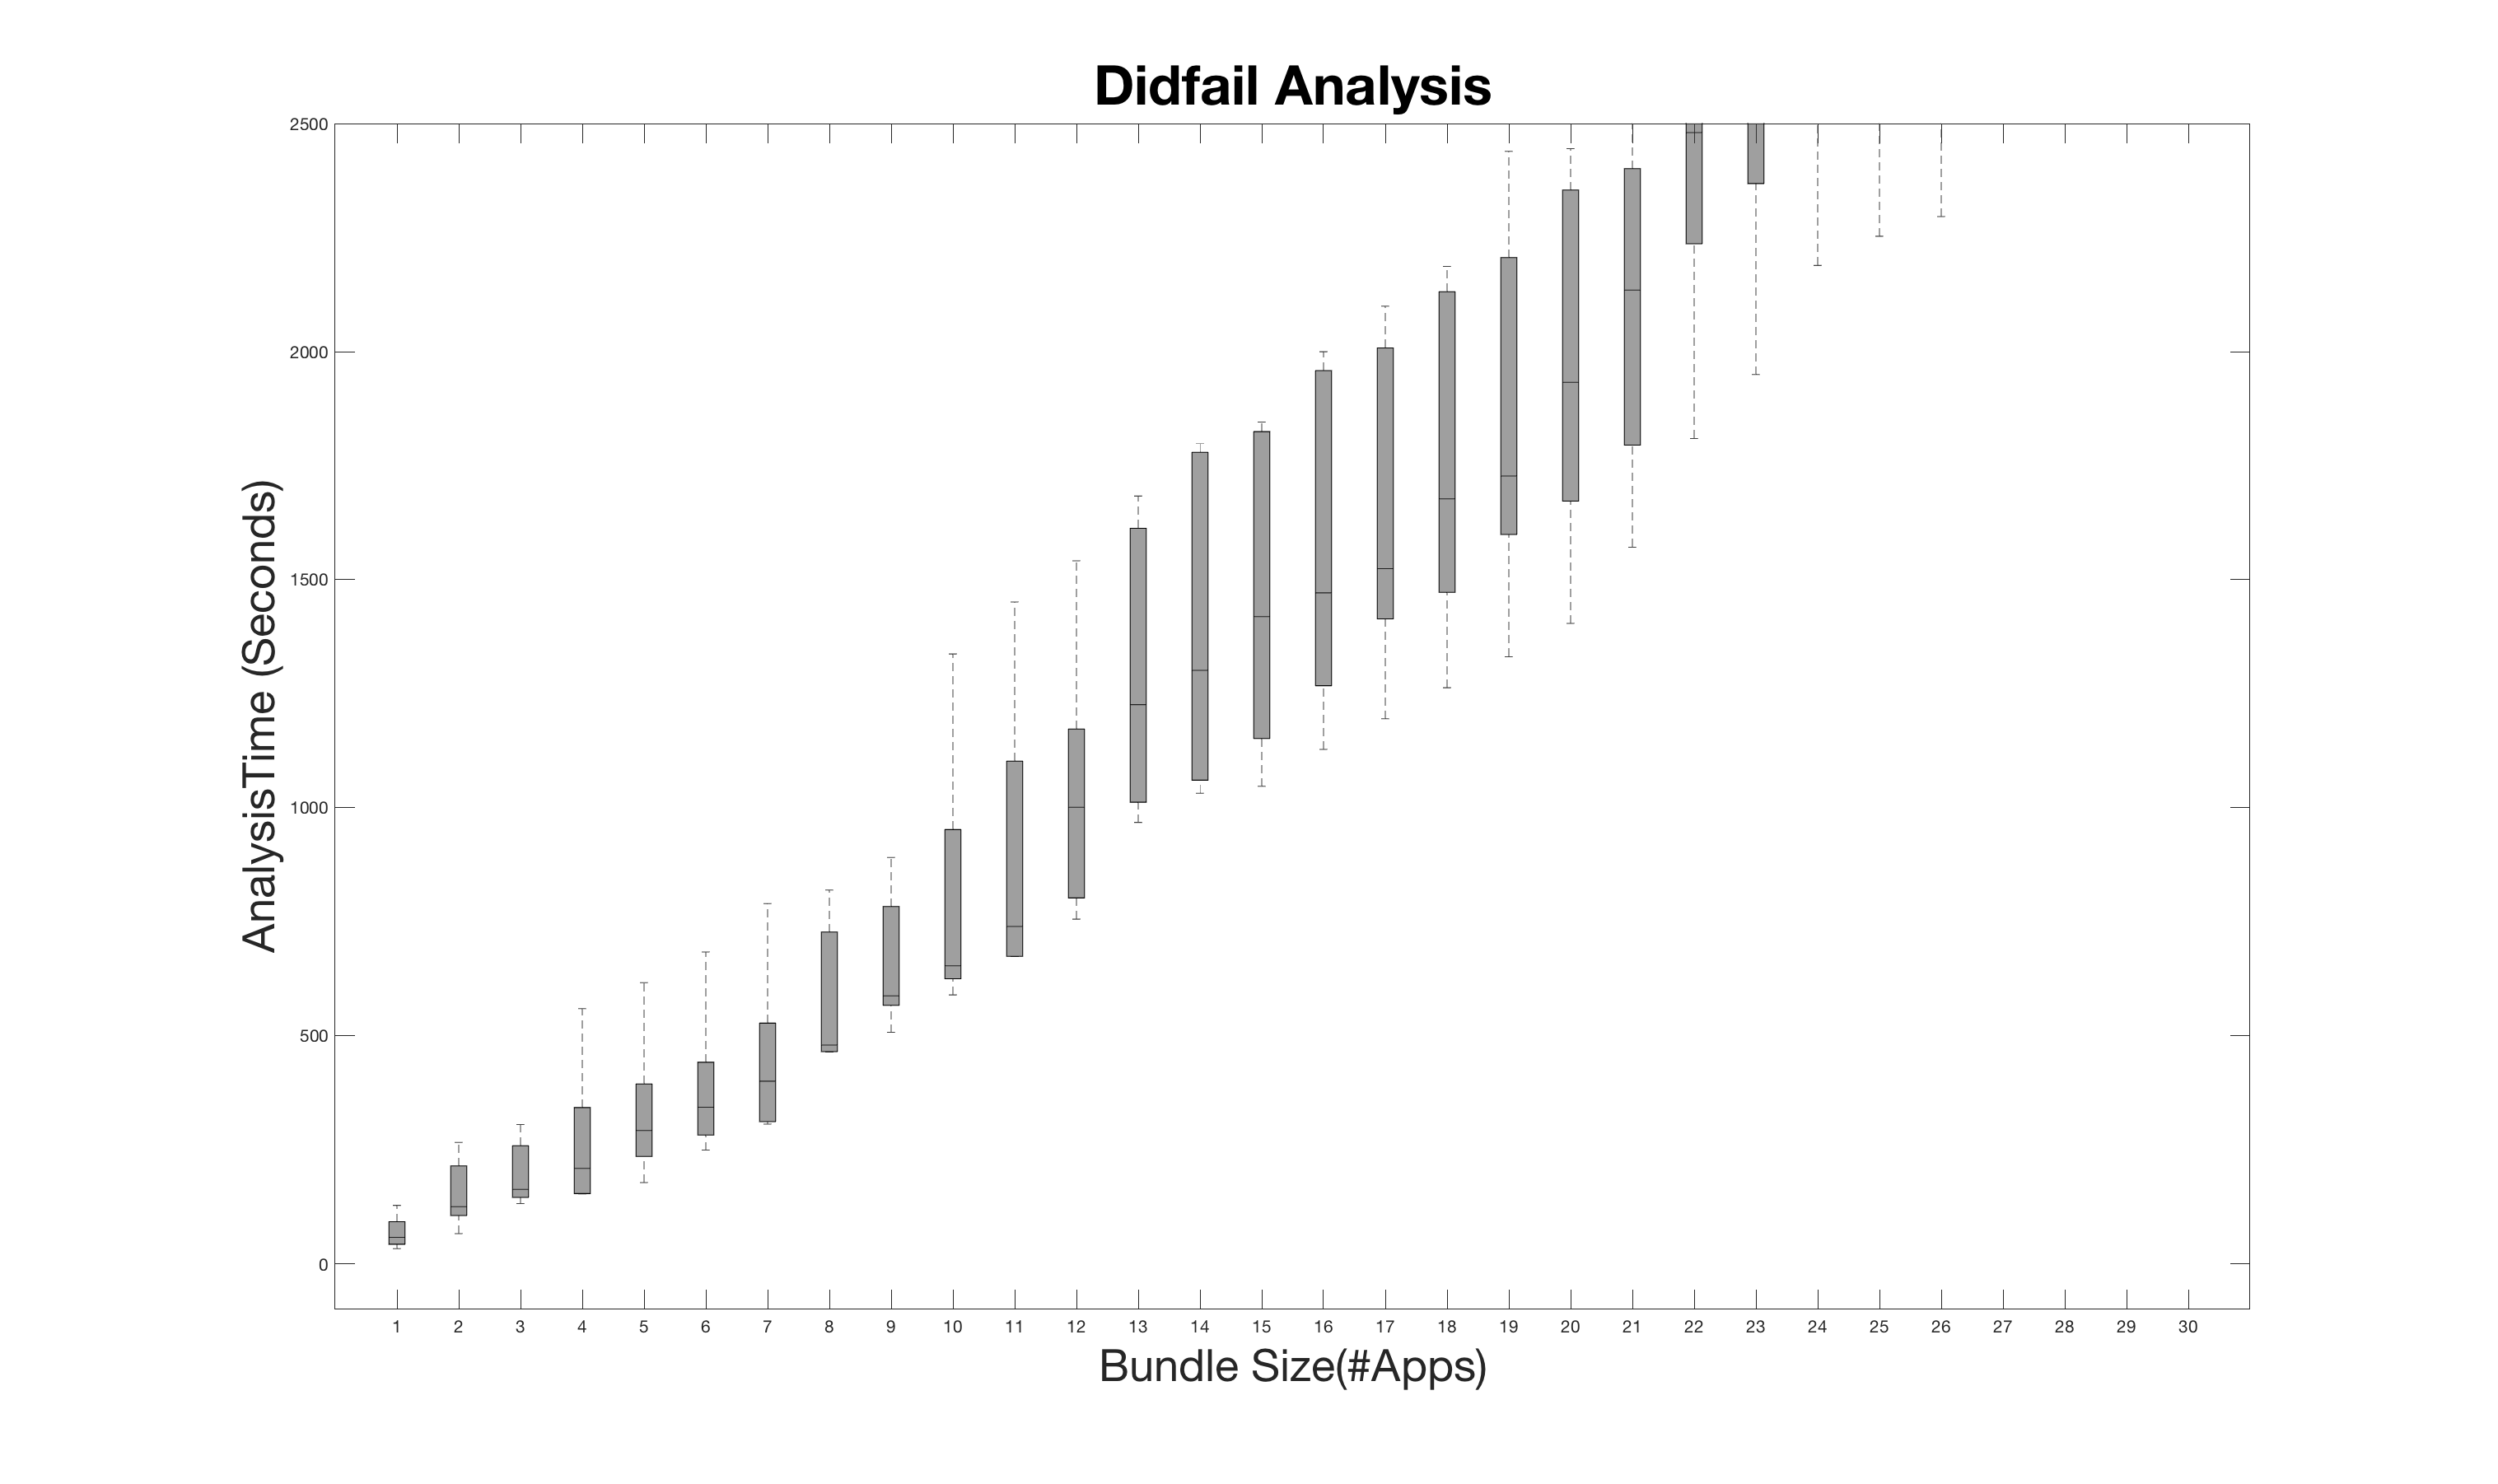
\includegraphics[width=\linewidth]{DidfailBoxPlot}
			\caption{Figure 1. This is a graph which shows Didfail's analysis times.}
		\end{figure}
	
	\subparagraph{DIALDroid}
		DIALDroid is an inter-application ICC security analysis tool with four key operations: ICC Entry / Exit Point Extraction, DataFlow Analysis, Data Aggregation, and ICC Leak Calculation.[1] DIALDroid extracts models from a given application and performs static analysis to find any ICC exit or entry leaks present. Then the information on any leaks is stored in a MySQL relational database to be retrieved when requested by SQL queries. During the initial analysis stage DIALDroid configures the precision based on the length of the analysis. During the first five minutes of analysis DIALDroid uses a high precision algorithm to find ICC entry and exit leaks. After five minutes DIALDroid switches to a low precision algorithm that has a higher change of false negative. If the analysis runs for more than a given timeout, such as 15 minutes, DIALDroid abandons the analysis of that application altogether.
	\subparagraph{SEALANT}
		Here is some text explain the tool Sealant.
\paragraph*{}
	To test each of these tools we used Oracle VirtualBox to create virtual machines running Ubuntu 16.04. For each tool the virtual machine was given the minimum amount of memory that we found it would run on. Covert, DidFail, and Flair all were given 3GB of memory, SEALANT was given 6GB, and DIALDroid, by far the most memory intensive, was given 14GB. Throughout all the tests The CPU was kept consistent at four physical cores and 8 threads. We found this to be the best way of testing each tool. Each tool was given enough memory to run efficiently, but none were given so much as to have a clear advantage over any other.\\ 
	We ran each tool against seven bundles of applications. Each bundle contained 50 popular android application.



\end{document}

